%\documentclass[dvisvgm]{minimal}
\documentclass{standalone}
\usepackage{fontspec}
\setmainfont{Linux Biolinum}
%\setmainfont{League Mono}
%\setmainfont{Fira Sans Condensed}
%\setmainfont{Gargoyle Mono}

\usepackage{tikz}
\usepackage{xcolor}
\begin{document}
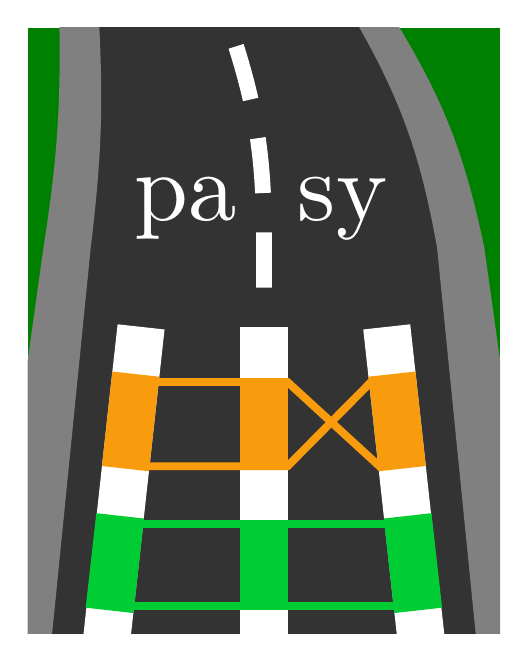
\begin{tikzpicture}

\clip  (-3, -4.9) rectangle (3, 2.8); % limit img size

\draw[draw opacity = 0, fill=green!50!black] (-3, -4.9) rectangle (3, 2.8);

% road
	\draw[fill=black!80, draw opacity=0]
	(3, -5)
	to (2.3, 0)
	to [bend right=10] (1.3, 3)
	to (-2.3, 3)
to [bend left=10] (-2.3, 0)
	to (-3, -5) --cycle;

	% footpaths
	\draw[draw opacity=0, fill=black!50]%, line width=.6cm, fill=black!80]
	(3.5, -5) to (2.7, -5) to (2.2, 0)
	to [bend right=10] (1.1, 3) to (1.6, 3)
	to [bend left=10] (2.8, 0) --cycle;

	\draw[draw opacity=0, fill=black!50]%, line width=.6cm, fill=black!80]
	(-3.5, -5) to (-2.7, -5) to (-2.2, 0)
	to [bend right=5] (-2.1, 3) to (-2.6, 3)
	to [bend left=5] (-2.8, 0) --cycle;

%	\draw[line width=.6cm, color=black!80]
%	(-3, -5)
%	to (-2.3, 0)
%	to [bend right=10] (-2.3, 3);

	% centre line
	\draw[color=white, line width=.2cm, dash= on .7cm off .5cm phase .7cm] (0, -1) to (0, 0) to [bend right=10] (-0.5, 3);

	% pasy name
	\node[scale=3.5, color=white] at (-1, 0.5){pa};
	\node[scale=3.5, color=white] at (1, 0.5){sy};

	% zebra strips
	\draw[color=white, line width=.6cm] (-2, -5) to (-1.56, -1);
	\draw[color=white, line width=.6cm] (0, -5) to (0, -1);
	\draw[color=white, line width=.6cm] (2, -5) to (1.56, -1);

	\newcommand{\coresyn}{blue!20!green}
	% core synteny
	\draw[line width=.1cm, color=\coresyn] (1.93, -4.55) to (0, -4.55) to (-1.93, -4.55);
	\draw[line width=.1cm, color=\coresyn] (1.89, -3.5) to (0, -3.5) to (-1.89, -3.5);
	\draw[line width=.61cm, color=\coresyn] (-1.96, -4.6) to (-1.825, -3.4);
	\draw[line width=.61cm, color=\coresyn] (1.96, -4.6) to (1.825, -3.4);
	\draw[line width=.61cm, color=\coresyn] (0, -4.6) to (0, -3.45);

	% cross synteny
	\newcommand{\crossyn}{yellow!60!red}
	\draw[line width=.1cm, color=\crossyn] (-1.5, -1.7) to (.3, -1.7) to (1.5, -2.8);
	\draw[line width=.1cm, color=\crossyn] (-1.6, -2.77) to (.3, -2.77) to (1.4, -1.66);
	\draw[line width=.6cm, color=\crossyn] (-1.758, -2.8) to (-1.626, -1.6);
	\draw[line width=.6cm, color=\crossyn] (1.758, -2.8) to (1.626, -1.6);
	\draw[line width=.6cm, color=\crossyn] (0, -2.8) to (0, -1.65);

	\end{tikzpicture}
\end{document}
